\subsection{GMM vs supervectors}

[GMM vs supervectors] Chosen system was adapt-kmeans

\begin{figure}[H]
	\centering
	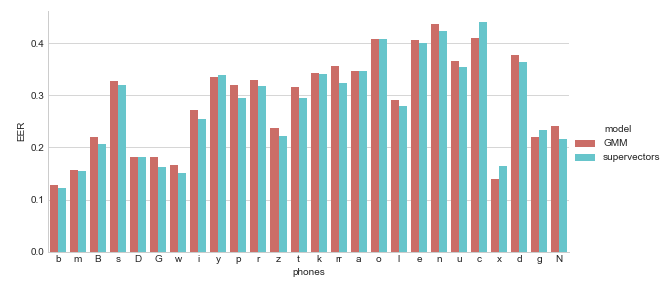
\includegraphics[width=0.6\textwidth]{files/figures/results/gmm-vs-supervectors/gmm-vs-supervectors-dev.png}
\end{figure}

\begin{figure}[H]
	\centering
	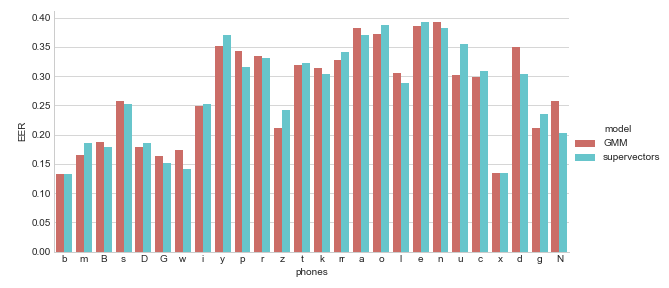
\includegraphics[width=0.6\textwidth]{files/figures/results/gmm-vs-supervectors/gmm-vs-supervectors-heldout.png}
\end{figure}


\subsection{Legendre and DCT}

\begin{figure}[H]
	\centering
	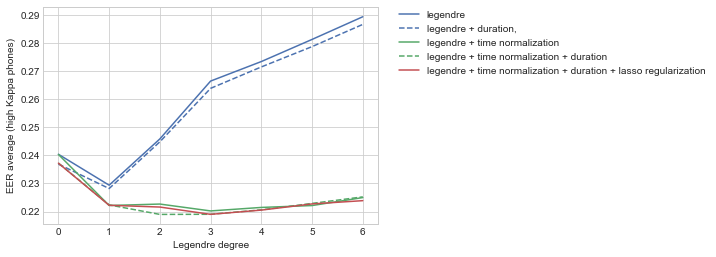
\includegraphics[width=0.8\textwidth]{files/figures/results/legendre-dct/legendre-tunning.png}
\end{figure}


\begin{figure}[H]
	\centering
	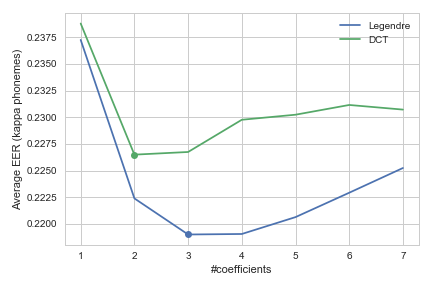
\includegraphics[width=0.5\textwidth]{files/figures/results/legendre-dct/legendre-dct-coefficients.png}
\end{figure}


\subsection{Fusion systems}

\begin{figure}[H]
	\centering
	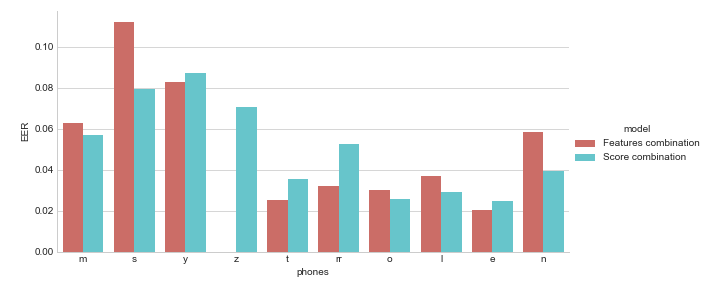
\includegraphics[width=0.6\textwidth]{files/figures/results/relatives/relatives-fusion-systems-dev-kappa.png}
\end{figure}

\begin{figure}[H]
	\centering
	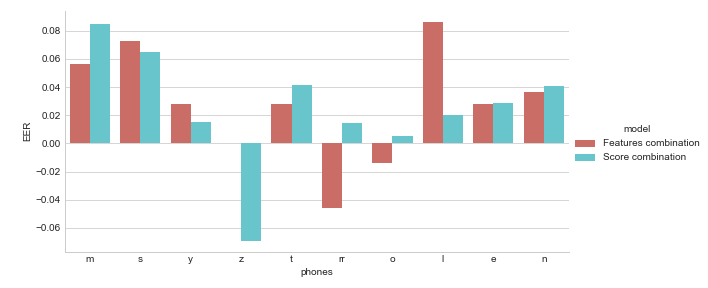
\includegraphics[width=0.6\textwidth]{files/figures/results/relatives/relative-fusion-systems-heldout-kappa.png}
\end{figure}
